\documentclass[12pt]{article}
\usepackage[margin=0.8in]{geometry}
\usepackage[utf8]{inputenc}
\usepackage{graphicx}
\usepackage[export]{adjustbox}
\usepackage{amsmath}
\usepackage{amsfonts}
\usepackage{amssymb}
\usepackage[version=4]{mhchem}
\usepackage{stmaryrd}
\usepackage{bbold}
%\usepackage[fallback]{xeCJK}
\usepackage{polyglossia}
\usepackage{fontspec}
\usepackage{censor}
%\setCJKmainfont{Noto Serif CJK TC}
\graphicspath{ {../Images/} }
\usepackage{enumitem}
\usepackage{tikz}
\usepackage{amsthm}
\usepackage{tcolorbox}
\usepackage{array}
\usepackage{tabularray}
\usepackage{makecell}
\usepackage{esvect}

\tcbuselibrary{theorems}

\definecolor{GrayCen}{HTML}{d2d2d2}
\definecolor{GrayBG}{HTML}{d9d9d9}
\definecolor{BlueDef}{HTML}{104e8b}
\definecolor{GreenProp}{HTML}{025540}
\definecolor{RedMet}{HTML}{cd5556}
\definecolor{BlackSav}{HTML}{000000}
\def\censorcolor{GrayCen}
\let\svcensorrule\censorrule
\renewcommand\censorrule[1]{%
\textcolor{\censorcolor}{\svcensorrule{#1}}}

\newtcbtheorem
[]% init options
{definition}% name
{Définition}% title
{%
  colback=GrayBG,
  colframe=BlueDef,
  fonttitle=\bfseries,
}% options
{def}% prefix

\newtcbtheorem
[]% init options
{proposition}% name
{Proposition}% title
{%
  colback=GrayBG,
  colframe=GreenProp,
  fonttitle=\bfseries,
}% options
{prop}% prefix

\newtcbtheorem
[]% init options
{method}% name
{Méthode}% title
{%
  theorem name,
  colback=GrayBG,
  colframe=RedMet,
  fonttitle=\bfseries,
}% options
{met}% prefix

\newtcbtheorem
[]% init options
{savoir}% name
{Savoir-faire du chapitre}% title
{%
  theorem name,
  colback=GrayBG,
  colframe=BlackSav,
  fonttitle=\bfseries,
}% options
{sav}% prefix

\newtheoremstyle{break}
{\topsep}{\topsep}%
{}{}%
{\bfseries}{}%
{\newline}{}%
\theoremstyle{break}
\newtheorem*{example}{Exemple.}
\newtheorem*{remark}{Remarque.}

\newenvironment{demo}[1][\proofname]{%
  \begin{proof}[#1]$ $\newline
  }{%
  \end{proof}
}

\setmainlanguage{french}
%\setmainfont{CMU Serif}

\title{
  \vspace{4em}
  \centering
  \tcbset{colframe=BlackSav,colback=GrayBG}
  \tcbox[tikznode]{
    Chapitre 7 \\Produit scalaire
  }
}

\author{}
\date{}

\setlength\parindent{0pt}
%\setlist[itemize]{topsep=0pt}
\setlist{nolistsep}
%\setlist[itemize]{noitemsep}
%\setlist[enumerate]{noitemsep}

\newcolumntype{C}[1]{>{\centering\arraybackslash}m{#1}}
\newcolumntype{L}[1]{>{\raggedright\arraybackslash}m{#1}}
\newcolumntype{N}{@{}m{0pt}@{}}

\begin{document}
\maketitle

\tableofcontents

%\newcommand{\hideM}[1]{\mbox{\vphantom{$#1$}\smash{\colorbox{gray!50}{$\displaystyle #1$}}} }
%\newcommand{\hide}[1]{\mbox{\vphantom{#1}\smash{\colorbox{gray!50}{#1}}}}
\newcommand{\hideM}[1]{\mbox{\vphantom{$#1$}\smash{\colorbox{gray!50}{\phantom{$\displaystyle #1$}}}} }
\newcommand{\hide}[1]{\mbox{\vphantom{#1}\smash{\colorbox{gray!50}{\phantom{#1}}}}}

\newpage

\section*{Introduction}
Le déterminant de deux vecteurs permet de savoir facilement s'ils sont colinéaires en utilisant la propriété suivante :

$$
\operatorname{det}(\vv{u} ; \vv{v})=0 \Longleftrightarrow \vv{u} \text { et } \vv{v} \text { sont colinéaires. }
$$

De manière similaire, l'objectif de ce chapitre est de définir une quantité permettant de savoir si deux vecteurs sont orthogonaux ou non. Plus précisément, on va définir le produit entre deux vecteurs $\vv{u}$ et $\vv{v}$, le résultat de ce produit étant un nombre réel égal à zéro si, et seulement si, les vecteurs sont orthogonaux.

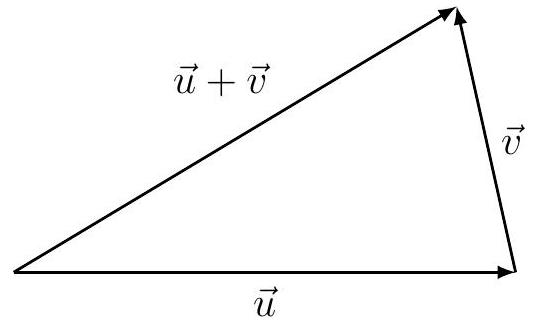
\includegraphics[width=0.3\textwidth, center]{2025_02_26_6fa51b4490e482ca532cg-2}

On considère les vecteurs $\vv{u}$ et $\vv{v}$ représentés sur la figure ci-dessus.\\
D'après le théorème de Pythagore :

$$
\begin{aligned}
  \vv{u} \text { et } \vv{v} \text { sont orthogonaux } & \Longleftrightarrow\|u+v\|^{2}=\|\vv{u}\|^{2}+\|\vv{v}\|^{2} \\
  & \Longleftrightarrow\|u+v\|^{2}-\|\vv{u}\|^{2}-\|\vv{v}\|^{2}=0
\end{aligned}
$$

On va donc définir, à quelque chose près, le produit de deux vecteurs comme étant égal à la quantité $\|\vv{u}+\vv{v}\|^{2}-\|\vv{u}\|^{2}-\|\vv{v}\|^{2}$.

Avec cette formule le produit d'un vecteur $\vv{u}$ par lui même serait toutefois égal à :

$$
\|u+u\|^{2}-\|\vv{u}\|^{2}-\|\vv{u}\|^{2}=\|2 \vv{u}\|^{2}-2\|\vv{u}\|^{2}=4\|\vv{u}\|^{2}-2\|\vv{u}\|^{2}=2\|\vv{u}\|^{2} .
$$

Il parait préférable que le produit d'un vecteur par lui même soit égal à $\|\vv{u}\|^{2}$ (cela permettra d'utiliser le produit de deux vecteurs non seulement pour tester l'orthogonalité de deux vecteurs mais aussi pour calculer des longueurs). C'est pourquoi nous allons ajouter un facteur $\dfrac{1}{2}$ à la formule précédente et définir le produit de $\vv{u}$ et $\vv{v}$ comme suit :

$$
\vv{u} \cdot \vv{v}=\dfrac{1}{2}\left(\|\vv{u}+\vv{v}\|^{2}-\|\vv{u}\|^{2}-\|\vv{v}\|^{2}\right) .
$$

\newpage

\section{Définitions et premières propriétés}
\begin{definition}{}{}
  On appelle produit scalaire de deux vecteurs $\vv{u}$ et $\vv{v}$, le réel noté $\vv{u} . \vv{v}$ et défini par

  $$
  \vv{u} \cdot \vv{v}=\dfrac{1}{2}\left(\|\vv{u}+\vv{v}\|^{2}-\|\vv{u}\|^{2}-\|\vv{v}\|^{2}\right)
  $$
\end{definition}

\begin{definition}{}{}
  Deux vecteurs non nuls sont dit ortogonaux si, et seulement si, $(\vv{u}, \vv{v})=\dfrac{\pi}{2}$ ou $(\vv{u}, \vv{v})=-\dfrac{\pi}{2}$
\end{definition}

\begin{remark}
  Par convention, le vecteur nul est orthogonal à tous les vecteurs du plan.
\end{remark}

\begin{proposition}{}{}
  $\vv{u}$ et $\vv{v}$ sont ortogonaux si, et seulement si, $\vv{u} \cdot \vv{v}=0$.
\end{proposition}

\begin{demo}
  Cela découle directement du théorème de Pythagore comme expliqué en introduction.
\end{demo}

\begin{proposition}{}{}
  Pour tout vecteur $\vv{u}$,

  $$
  \vv{u} \cdot \vv{u}=\|\vv{u}\|^{2}
  $$
\end{proposition}

\begin{remark}
  On note $\vv{u} \cdot \vv{u}=\vv{u}^{2}$ que l'on appelle carré scalaire de $\vv{u}$.
\end{remark}
\begin{demo}
  \begin{align*}
    \vv{u} \cdot \vv{u}=\dfrac{1}{2}\left(\|u+u\|^{2}-\|\vv{u}\|^{2}-\|\vv{u}\|^{2}\right)=\dfrac{1}{2}\left(\|2 \vv{u}\|^{2}-2\|\vv{u}\|^{2}\right)=\dfrac{1}{2}\left(4\|\vv{u}\|^{2}-2\|\vv{u}\|^{2}\right)&=\dfrac{1}{2}\left(2\|\vv{u}\|^{2}\right)\\
    &=\|\vv{u}\|^{2}.
  \end{align*}
\end{demo}

\section{Propriétés algébriques du produit scalaire}
\subsection{Formule avec les coordonnées}
\begin{proposition}{}{}
  Soient $\vv{u}\dbinom{x}{y}$ et $\vv{v}\dbinom{x^{\prime}}{y^{\prime}}$ dans un repère orthonormé. Alors

  $$
  \vv{u} \cdot \vv{v}=x x^{\prime}+y y^{\prime}
  $$
\end{proposition}

\begin{demo}
  $$
  \begin{aligned}
    \vv{u} . \vv{v} & =\dfrac{1}{2}\left(\|\vv{u}+\vv{v}\|^{2}-\|\vv{u}\|^{2}-\|\vv{v}\|^{2}\right) \\
    & =\dfrac{1}{2}\left(\left(x+x^{\prime}\right)^{2}+\left(y+y^{\prime}\right)^{2}-\left(x^{2}+y^{2}\right)-\left(x^{\prime 2}+y^{\prime 2}\right)\right) \\
    & =\dfrac{1}{2}\left(2 x x^{\prime}+2 y y^{\prime}\right) \\
    & =x x^{\prime}+y y^{\prime} .
  \end{aligned}
  $$
\end{demo}

\begin{example}
  Les vecteurs $\vv{u}\dbinom{1}{-2}$ et $\vv{v}\dbinom{4}{2}$ sont orthogonaux car $\vv{u} \cdot \vv{v}=1 \times 4+(-2) \times 2=0$.
\end{example}

\subsection{Symétrie et bilinéarité}
\begin{proposition}{}{}
  Le produit scalaire est symétrique (on dit aussi commutatif), c'est-à-dire que pour tous $\vv{u}$ et $\vv{v}$,

  $$
  \vv{u} \cdot \vv{v}=\vv{v} \cdot \vv{u}
  $$
\end{proposition}

\begin{demo}
  Il suffit d'utiliser la formule avec les coordonnées (propriété 2.1). On a :

  $$
  \vv{u} \cdot \vv{v}=x x^{\prime}+y y^{\prime}=x^{\prime} x+y^{\prime} y=\vv{v} \cdot \vv{u}
  $$
\end{demo}

\begin{proposition}{}{}
  Le produit scalaire est bilinéaire, c'est à dire que pour tous vecteurs $\vv{u}, \vv{v}$ et $\vv{w}$, et pour tout réel $k$ :

  \begin{itemize}
    \item $\vv{u} \cdot(\vv{v}+\vv{w})=\vv{u} \cdot \vv{v}+\vv{u} \cdot \vv{w}$
    \item $(k \vv{u}) \cdot \vv{v}=\vv{u} \cdot(k \vv{v})=k(\vv{u} \cdot \vv{v})$
  \end{itemize}
\end{proposition}

\begin{demo}
  On note $\vv{u}\dbinom{x}{y}, \vv{v}\dbinom{x^{\prime}}{y^{\prime}}$ et $\vv{w}\dbinom{x^{\prime \prime}}{y^{\prime \prime}}$ les coordonnées dans un repère orthonormé.

  \begin{itemize}
    \item D'une part, d'après la formule du produit scalaire avec les coordonnées, $\vv{u} .(v+\vv{w})=x\left(x^{\prime}+x^{\prime \prime}\right)+y\left(y^{\prime}+y^{\prime \prime}\right)=x x^{\prime}+x x^{\prime \prime}+y y^{\prime}+y y^{\prime \prime}$.\\
      D'autre part, $\vv{u} \cdot \vv{v}+\vv{u} \cdot \vv{w}=x x^{\prime}+y y^{\prime}+x x^{\prime \prime}+y y^{\prime \prime}$, ce qui prouve l'égalité.
    \item D'une part, $(k \vv{u}) \cdot \vv{v}=(k x) \times x^{\prime}+(k y) \times y^{\prime}=k x x^{\prime}+k y y^{\prime}$.\\
      D'autre part, $\vv{u} .(k \vv{v})=x \times\left(k x^{\prime}\right)+y \times\left(k y^{\prime}\right)=k x x^{\prime}+k y y^{\prime}$\\
      Enfin, $k(\vv{u} . \vv{v})=k\left(x x^{\prime}+y y^{\prime}\right)=k x x^{\prime}+k y y^{\prime}$.\\
      On voit donc que les trois quantités sont bien égales.
  \end{itemize}
\end{demo}

\subsection{Identités remarquables}
\begin{proposition}{}{}
  \begin{itemize}
    \item $\|\vv{u}+\vv{v}\|^{2}=\|\vv{u}\|^{2}+2 \vv{u} \cdot \vv{v}+\|\vv{v}\|^{2}$
    \item $\|\vv{u}-\vv{v}\|^{2}=\|\vv{u}\|^{2}-2 \vv{u} \cdot \vv{v}+\|\vv{v}\|^{2}$
    \item $(\vv{u}-\vv{v}) \cdot(\vv{u}+\vv{v})=\|\vv{u}\|^{2}-\|\vv{v}\|^{2}$
  \end{itemize}
\end{proposition}
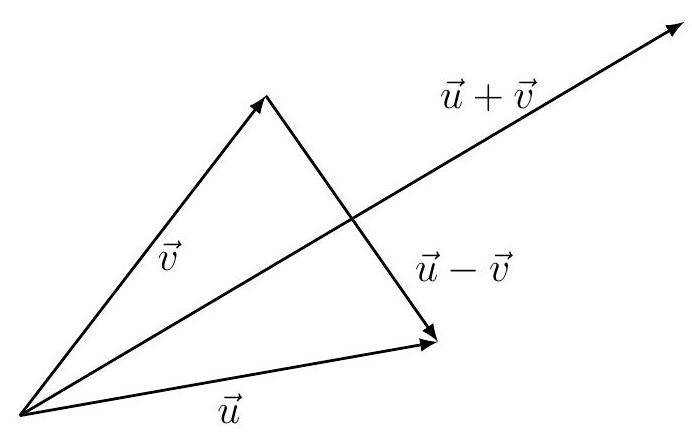
\includegraphics[width=0.5\textwidth, center]{2025_02_26_6fa51b4490e482ca532cg-5}

\begin{demo}
  \vspace{-1em}
  \begin{itemize}
    \item Cette égalité découle directement de la définition du produit scalaire (définition 1).
    \item Pour montrer cette égalité, on applique la première égalité aux vecteurs $\vv{u}$ et $-\vv{v}$.
    \item Pour montrer cette égalité, il suffit de développer en utilisant la bilinéarité du produit scalaire.
  \end{itemize}
\end{demo}

\begin{proposition}{}{}
  \begin{itemize}[itemsep=5pt]
    \item $\vv{u} \cdot \vv{v}=\frac{1}{2}\left(\|\vv{u}+\vv{v}\|^{2}-\|\vv{u}\|^{2}-\|\vv{v}\|^{2}\right)$
    \item $\vv{u} \cdot \vv{v}=\frac{1}{2}\left(\|\vv{u}\|^{2}+\|\vv{v}\|^{2}-\|\vv{u}-\vv{v}\|^{2}\right)$
    \item $\vv{u} \cdot \vv{v}=\frac{1}{4}\left(\|\vv{u}+\vv{v}\|^{2}-\|\vv{u}-\vv{v}\|^{2}\right)$
  \end{itemize}
\end{proposition}

\begin{demo}
  \vspace{-1em}
  \begin{itemize}
    \item Cette égalité est simplement un rappel de la définition du produit scalaire (définition 1).
    \item Cette égalité découle directement de la deuxième égalité de la propriété 2.3.
    \item Pour montrer cette égalité, il suffit de faire la moyenne de deux premières égalités.
  \end{itemize}
\end{demo}

\section{Propriétés géométriques du produit scalaire}
\subsection{Formule trigonométrique}
\begin{proposition}{}{}
  Pour tous vecteurs $\vv{u}$ et $\vv{v}$, si $\theta=(\vv{u}, \vv{v})$ alors :

  $$
  \vv{u} . \vv{v}=\|\vv{u}\| \times\|\vv{v}\| \times \cos (\theta)
  $$
\end{proposition}

\begin{center}
  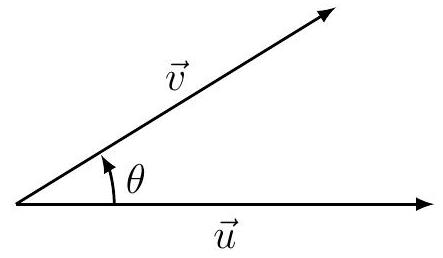
\includegraphics[width=0.25\textwidth]{2025_02_26_6fa51b4490e482ca532cg-6(1)}
\end{center}

\begin{remark}
  Avec cette formule, on retrouve le fait que pour tous vecteurs non nuls $\vv{u}$ et $\vv{v}, \vv{u} \cdot \vv{v}=0$ si, et seulement si, $(\vv{u}, \vv{v})=\dfrac{\pi}{2} \quad$ ou $\quad(\vv{u}, \vv{v})=\dfrac{-\pi}{2}$.
\end{remark}

\begin{demo}
  Soient deux vecteurs $\vv{u}$ et $\vv{v}$. On définit le repère orthonormé $(0 ; \vv{i}, \vv{j})$ tel que $\vv{i}=\dfrac{1}{\|\overrightarrow{\|}\|} \vv{u}$ et tel que $(\vv{i} ; \vv{j})=+\dfrac{\pi}{2}$. Dans ce repère, $\vv{v}$ a pour coordonnées $\dbinom{\|\vv{v}\| \cos \theta}{\|\vv{v}\| \sin \theta}$.\\
  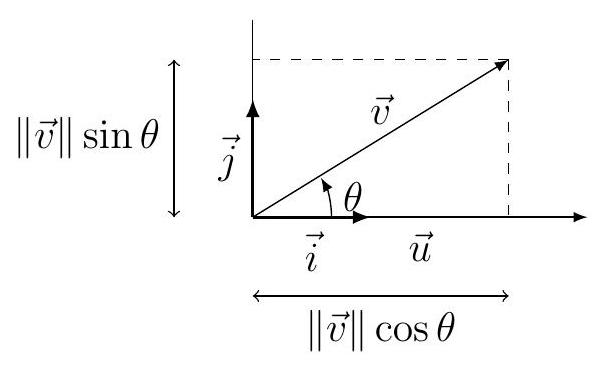
\includegraphics[width=0.4\textwidth, center]{2025_02_26_6fa51b4490e482ca532cg-6}

  Étant donné que le vecteur $\vv{u}$ a pour coordonnées $\dbinom{\|\vv{u}\|}{0}$, on voit, d'après la formule en fonction des coordonnées que

  $$
  \vv{u} \cdot \vv{v}=\|\vv{u}\| \times\|\vv{v}\| \cos (\theta)+0 \times\|\vv{v}\| \sin \theta=\|\vv{u}\|\|\vv{v}\| \cos (\theta) .
  $$
\end{demo}

\subsection{Formule du projeté orthogonal}
\begin{proposition}{}{}
  Soient $\overrightarrow{A B}$ et $\overrightarrow{A C}$ deux vecteurs et soit $H$ le projeté orthogonal du point $C$ sur la droite (AB). Alors,

  $$
  \overrightarrow{\mathrm{AB}} \cdot \overrightarrow{\mathrm{AC}}=\overrightarrow{\mathrm{AB}} \cdot \overrightarrow{\mathrm{AH}}=\left\{
    \begin{array}{cl}
      \mathrm{AB} \times \mathrm{AH} & \text { si } \overrightarrow{\mathrm{AB}} \text { et } \overrightarrow{\mathrm{AH}} \text { sont de même sens. } \\
      -\mathrm{AB} \times \mathrm{AH} &
      \text { sinon }
    \end{array}\right.
    $$
  \end{proposition}

  \begin{center}
    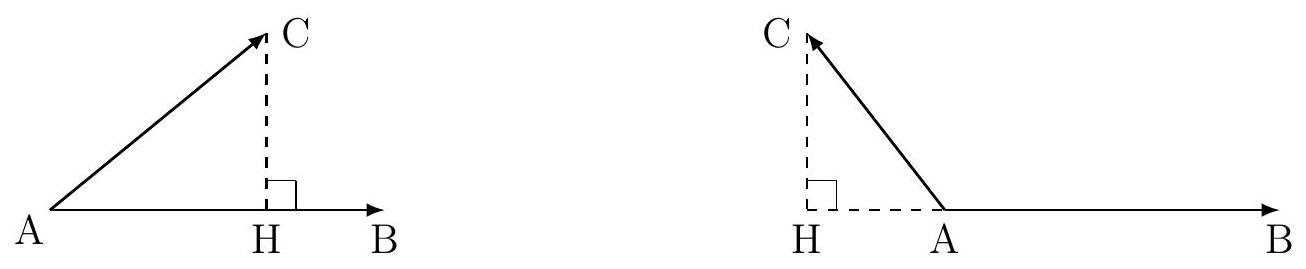
\includegraphics[max width=0.8\textwidth]{2025_02_26_6fa51b4490e482ca532cg-6(2)}
  \end{center}

  \begin{demo}
    $$
    \begin{aligned}
      \overrightarrow{\mathrm{AB}} \cdot \overrightarrow{\mathrm{AC}} & =\overrightarrow{\mathrm{AB}} \cdot(\overrightarrow{\mathrm{AH}}+\overrightarrow{\mathrm{HC}}) \\
      & =\overrightarrow{\mathrm{AB}} \cdot \overrightarrow{\mathrm{AH}}+\overrightarrow{\mathrm{AB}} \cdot \overrightarrow{\mathrm{HC}} \\
      & =\overrightarrow{\mathrm{AB}} \cdot \overrightarrow{\mathrm{AH}}(\operatorname{car} \overrightarrow{\mathrm{AB}} \text { et } \overrightarrow{\mathrm{HC}} \text { sont orthogonaux }) \\
      & =\mathrm{AB} \times \mathrm{AH} \times \cos (\overrightarrow{\mathrm{AB}} ; \overrightarrow{\mathrm{HB}})
    \end{aligned}
    $$

    On conclut ensuite en remarquant que $\overrightarrow{\mathrm{AB}}$ et $\overrightarrow{\mathrm{AH}}$ sont colinéaires donc $\cos (\overrightarrow{\mathrm{AB}} ; \overrightarrow{\mathrm{AH}})=1$ ou $\cos (\overrightarrow{\mathrm{AB}} ; \overrightarrow{\mathrm{AH}})=-1$.
  \end{demo}

  \begin{savoir}{}{}
    \begin{itemize}
      \item Calculer le produit scalaire de deux vecteurs en choisissant une méthode adaptée.
      \item Utiliser le produit scalaire pour démontrer une orthogonalité, calculer un angle ou calculer une longueur.
    \end{itemize}
  \end{savoir}

  \end{document}